\chapter{Testing}

To check the accuracy and performance of the add-on, we used malware web pages and benign web pages. To create malware samples, we generated different variants of Transcriptase malware. For benign web pages, we retrieved the JavaScript dead code from http://tools.w3clubs.com/jojo/.

Entire testing is performed on a system with the configuration specified in Table \ref{tab:title}:
\begin {table}[h]
\caption {System Specifications} \label{tab:title} 
  \begin{tabular}{|c|c|} 
\midrule
System Model & MacBook Pro (Retina, 13-inch, Mid 2014)\\
\midrule
Processor & 2.8 GHz Intel Core i5\\
\midrule
RAM & 16 GB 1600 MHz DDR3\\
\midrule
Storage & 120 GB\\
\midrule
Firefox version & 36.0.4\\
\midrule
SDK version & Add-on SDK 1.17\\
\midrule
Rhino version & Rhino 1.7R4, modified to output opcodes during JS compilation\\
\midrule
Java version & 1.7.0\_71\\
\midrule
\end{tabular}
 \end {table}

\section{Generating Transcriptase variants}

Transcriptase was written in JScript, so in windows system it can be executed by simply double clicking it. Generation of each version takes around 15 minutes. 

As explained in Section \ref{transcriptasesection}, Transcriptase carries its source code as meta instructions and on each execution it creates different variant of its JS source, then prepends that JS code to all the JavaScript files in its directory. So, I followed the below steps to create 100 versions:
\begin{enumerate}
\item Created an empty JavaScript file in Transcriptase directory
\item Executed Transcriptase, which infects the new empty JavaScript file and converts it to another variant of Transcriptase
\item Move the older version Transcriptase (or creator Transcriptase) to different folder.
\item Then created an empty JavaScript file in the current folder where the new Transcriptase variant exists.
\item Executed the new variant to infect the empty JavaScript file. Go to Step 3 if required number of variants aren`t generated. 
\end{enumerate}
Code in Figure \ref{fig:batchscriptcode} automates the above mentioned steps.

\begin{figure}[h]
  \centering
\begin{lstlisting}[frame=single,language=JavaScript,mathescape=false,morekeywords={REN, MOVE, IN, COPY, PAUSE, FOR, DO}]
FOR %%A IN (1 2 3 4 5 6 7 8 9 10 11 12 13 14 15 16 17 18 19 20 21 22 23 24 25 26 27 28 29 30 31 32 33 34 35 36 37 38 39 40 41 42 43 44 45 46 47 48 49 50 51 52 53 54 55 56 57 58 59 60 61 62 63 64 65 66 67 68 69 70 71 72 73 74 75 76 77 78 79 80 81 82 83 84 85 86 87 88 89 90 91 92 93 94 95 96 97 98 99 100) DO (
transcriptase.js
REN transcriptase.js "var%%~nA.*"
MOVE "var%%~nA.*" "C:\Users\Sravan\Downloads\Transcriptase\versions"
REN empty.js transcriptase.js
COPY "C:\Users\Sravan\Downloads\Transcriptase\template\empty.js" .
)
PAUSE
\end{lstlisting}
\caption[Batch script]{Batch script that automates the Transcriptase variants generations}
    \label{fig:batchscriptcode}
\end{figure}

\begin{figure}[h]
  \centering
      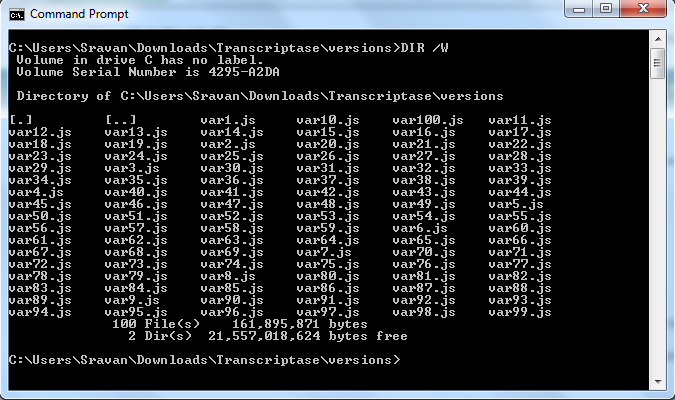
\includegraphics[width=16.875cm, height=10cm]{Capture.PNG}
    \caption[Transcriptase`s 100 versions]{Transcriptase`s 100 versions.}
    \label{fig:100versions}
\end{figure}

\section{Similarity scores and add-on performance}
Included console.log() functions in the add-on to log the following details - opcode similarity score and the add-on execution time taken to validate the web page. The below sub section deals with comparison of these details for benign and malware web pages. For testing add-on, we used 100 samples of benign web page and morphed malware web pages. Malware web pages are morphed by adding randomly generated junk code to it.
\subsection{Addition of 550 lines of dead code}
For this experiment, we used benign web page samples with 550 lines of junk code and also added the same amount of randomly generated junk code to malware web pages. Tables in Figures ~\ref{fig:b500table} and  ~\ref{fig:m500table} contains the details of scores and execution time for the benign and malware samples, respectively. From the table values, we can see that the scores for benign web pages are in the order of $10^{-3}$ whereas the scores for malware web pages are in the order of $10^{-4}$. Graph in Figure ~\ref{fig:bvsm500} clearly shows that the add-on is able to distinguish malware web pages and benign web pages correctly. Only 3 out of 100 malware samples have score similar to benign web pages.

\begin{figure}[h]
  \centering
  \begin{tabular}{|c|c|c|c|c|c|c|c|c|c|c|c|} 
  \midrule
 \begin{sideways}Score\end{sideways}& \begin{sideways}Time\end{sideways} \begin{sideways} (milliseconds)\end{sideways}& \begin{sideways}Score\end{sideways}& \begin{sideways}Time\end{sideways}  \begin{sideways}(milliseconds)\end{sideways}& \begin{sideways}Score\end{sideways}& \begin{sideways}Time\end{sideways}  \begin{sideways}(milliseconds)\end{sideways}& \begin{sideways}Score\end{sideways}& \begin{sideways}Time\end{sideways}  \begin{sideways} (milliseconds)\end{sideways}\\
\midrule
0.00147929&1136&0.00147929&1135&0.00147929&1482&0.0014792903&1232\\
\midrule
0.00147929&1172&0.0014792896&1124&0.0014792896&1304&0.0014792907&1115\\
\midrule
0.00147929&1150&0.0014792907&1113&0.00147929&1245&0.00147929&1308\\
\midrule
0.00147929&1125&0.0014792903&1178&0.0014792907&1274&0.0014792896&1159\\
\midrule
0.0014792893&1080&0.0014792896&1133&0.0014792896&1235&0.00147929&1125\\
\midrule
0.00147929&1223&0.0014792903&1133&0.0014792903&1242&0.0014792903&1228\\
\midrule
0.0014792896&1125&0.00147929&1134&0.0014792903&1246&0.0014792896&1180\\
\midrule
0.0014792903&1132&0.0014792893&1106&0.0014792903&1250&0.0014792893&1131\\
\midrule
0.001479291&1120&0.00147929&1142&0.0014792903&1257&0.00147929&1136\\
\midrule
0.0014792903&1198&0.0014792896&1159&0.0014792903&1255&0.0014792907&1132\\
\midrule
0.0014792903&1134&0.0014792896&1125&0.0014792903&1214&0.0014792896&1141\\
\midrule
0.0014792907&1131&0.0014792907&1122&0.0014792903&1152&0.00147929&1134\\
\midrule
0.0014792903&1108&0.00147929&1176&0.0014792896&1116&0.0014792896&1124\\
\midrule
0.00147929&1110&0.0014792903&1134&0.0014792907&1138&0.0014792903&1410\\
\midrule
0.00147929&1124&0.0014792893&1113&0.00147929&1105&0.0014792907&1123\\
\midrule
0.0014792893&1122&0.00147929&1168&0.0014792907&1093&0.00147929&1150\\
\midrule
0.0014792907&1116&0.00147929&1135&0.0014792903&1175&0.0014792903&1175\\
\midrule
0.0014792896&1117&0.0014792907&1118&0.0014792907&1121&0.0014792903&1116\\
\midrule
0.0014792903&1198&0.0014792903&1148&0.0014792903&1127&0.0014792893&1125\\
\midrule
0.00147929&1122&0.0014792907&1102&0.0014792903&1167&0.0014792896&1143\\
\midrule
0.00147929&1137&0.0014792893&1144&0.0014792903&1105&0.0014792903&1223\\
\midrule
0.00147929&1204&0.0014792896&1098&0.0014792907&1113&0.0014792903&1120\\
\midrule
0.0014792907&1130&0.00147929&1152&0.0014792896&1111&0.0014792907&1140\\
\midrule
0.00147929&1104&0.0014792903&1129&0.00147929&1140&0.00147929&1213\\
\midrule
0.0014792903&1119&0.00147929&1215&0.00147929&1149&0.00147929&1119\\
\midrule
\end{tabular}
    \caption[Scores table of benign web pages]{Table illustrating the scores and add-on execution time for 100 benign web pages, in four columns (i.e., 25 samples per column). Benign webpages are generated with 550 lines of dead code.}
    \label{fig:b500table}
\end{figure}
\begin{figure}[h]
  \centering
  \begin{tabular}{|c|c|c|c|c|c|c|c|c|c|c|c|} 
  \midrule
 \begin{sideways}Score\end{sideways}& \begin{sideways}Time\end{sideways} \begin{sideways} (milliseconds)\end{sideways}& \begin{sideways}Score\end{sideways}& \begin{sideways}Time\end{sideways}  \begin{sideways}(milliseconds)\end{sideways}& \begin{sideways}Score\end{sideways}& \begin{sideways}Time\end{sideways}  \begin{sideways}(milliseconds)\end{sideways}& \begin{sideways}Score\end{sideways}& \begin{sideways}Time\end{sideways}  \begin{sideways} (milliseconds)\end{sideways}\\
\midrule
0.00036982258&7897&0.00036982243&6707&0.00036982258&7888&0.0003698225&6642\\
\midrule
0.00036982258&6875&0.001423994&7493&0.00036982243&8133&0.00036982234&7355\\
\midrule
0.00036982258&6284&0.0003698224&6041&0.0003698224&8576&0.00036982235&7489\\
\midrule
0.0014239943&6430&0.00036982266&7119&0.00036982258&7785&0.00036982266&7072\\
\midrule
0.00036982234&7629&0.0003698225&7223&0.00036982243&8536&0.00036982258&6941\\
\midrule
0.00036982238&7682&0.00036982258&7159&0.00036982234&7118&0.0003698225&7372\\
\midrule
0.00036982266&7774&0.0003698225&8297&0.0003698225&7138&0.00036982243&7832\\
\midrule
0.00036982266&8075&0.00036982243&6949&0.00036982243&6917&0.00036982258&7158\\
\midrule
0.0003698225&6127&0.00036982243&8550&0.00036982243&6475&0.00036982258&6603\\
\midrule
0.00036982258&7312&0.0003698225&7157&0.00036982243&8109&0.0003698224&8482\\
\midrule
0.00036982258&8038&0.0003698225&7532&0.00036982258&7013&0.00036982243&7718\\
\midrule
0.00036982258&10123&0.0003698224&6904&0.00036982258&6740&0.00036982258&6723\\
\midrule
0.00036982236&8091&0.0003698225&6679&0.0003698225&7239&0.00036982258&8046\\
\midrule
0.00036982245&6392&0.00036982258&7031&0.0003698225&7138&0.0003698225&7845\\
\midrule
0.00036982238&6518&0.00036982258&6438&0.00036982258&6088&0.00036982258&7862\\
\midrule
0.00036982251&7121&0.00036982266&8230&0.00036982243&7529&0.00036982258&9817\\
\midrule
0.00036982243&6309&0.0003698225&9986&0.0003698224&8031&0.0003698224&7804\\
\midrule
0.00036982258&8646&0.0003698225&6958&0.0003698224&7753&0.0003698225&9849\\
\midrule
0.00036982243&6706&0.00036982243&10166&0.0014239943&6494&0.0003698225&9302\\
\midrule
0.00036982258&6617&0.0003698225&8358&0.00036982258&6815&0.00036982256&7239\\
\midrule
0.00036982241&6502&0.00036982251&6129&0.00036982266&8174&0.00036982263&7652\\
\midrule
0.00036982232&7289&0.00036982249&6732&0.00036982275&8314&0.0003698225&7261\\
\midrule
0.0003698224&7236&0.00036982258&7730&0.00036982266&7465&0.00036982258&6398\\
\midrule
0.00036982258&7746&0.00036982258&7719&0.00036982266&7113&0.0003698225&8812\\
\midrule
0.00036982243&7267&0.00036982258&7992&0.00036982258&6757&0.00036982243&8357\\
\midrule
\end{tabular}
    \caption[Scores table of malware web pages]{Table illustrating the scores and add-on execution time for 100 malware web pages, in four columns (i.e., 25 samples per column). Malware webpages are morphed with 550 lines of dead code. }
    \label{fig:m500table}
\end{figure}

\begin{figure}[h]
    \centering
    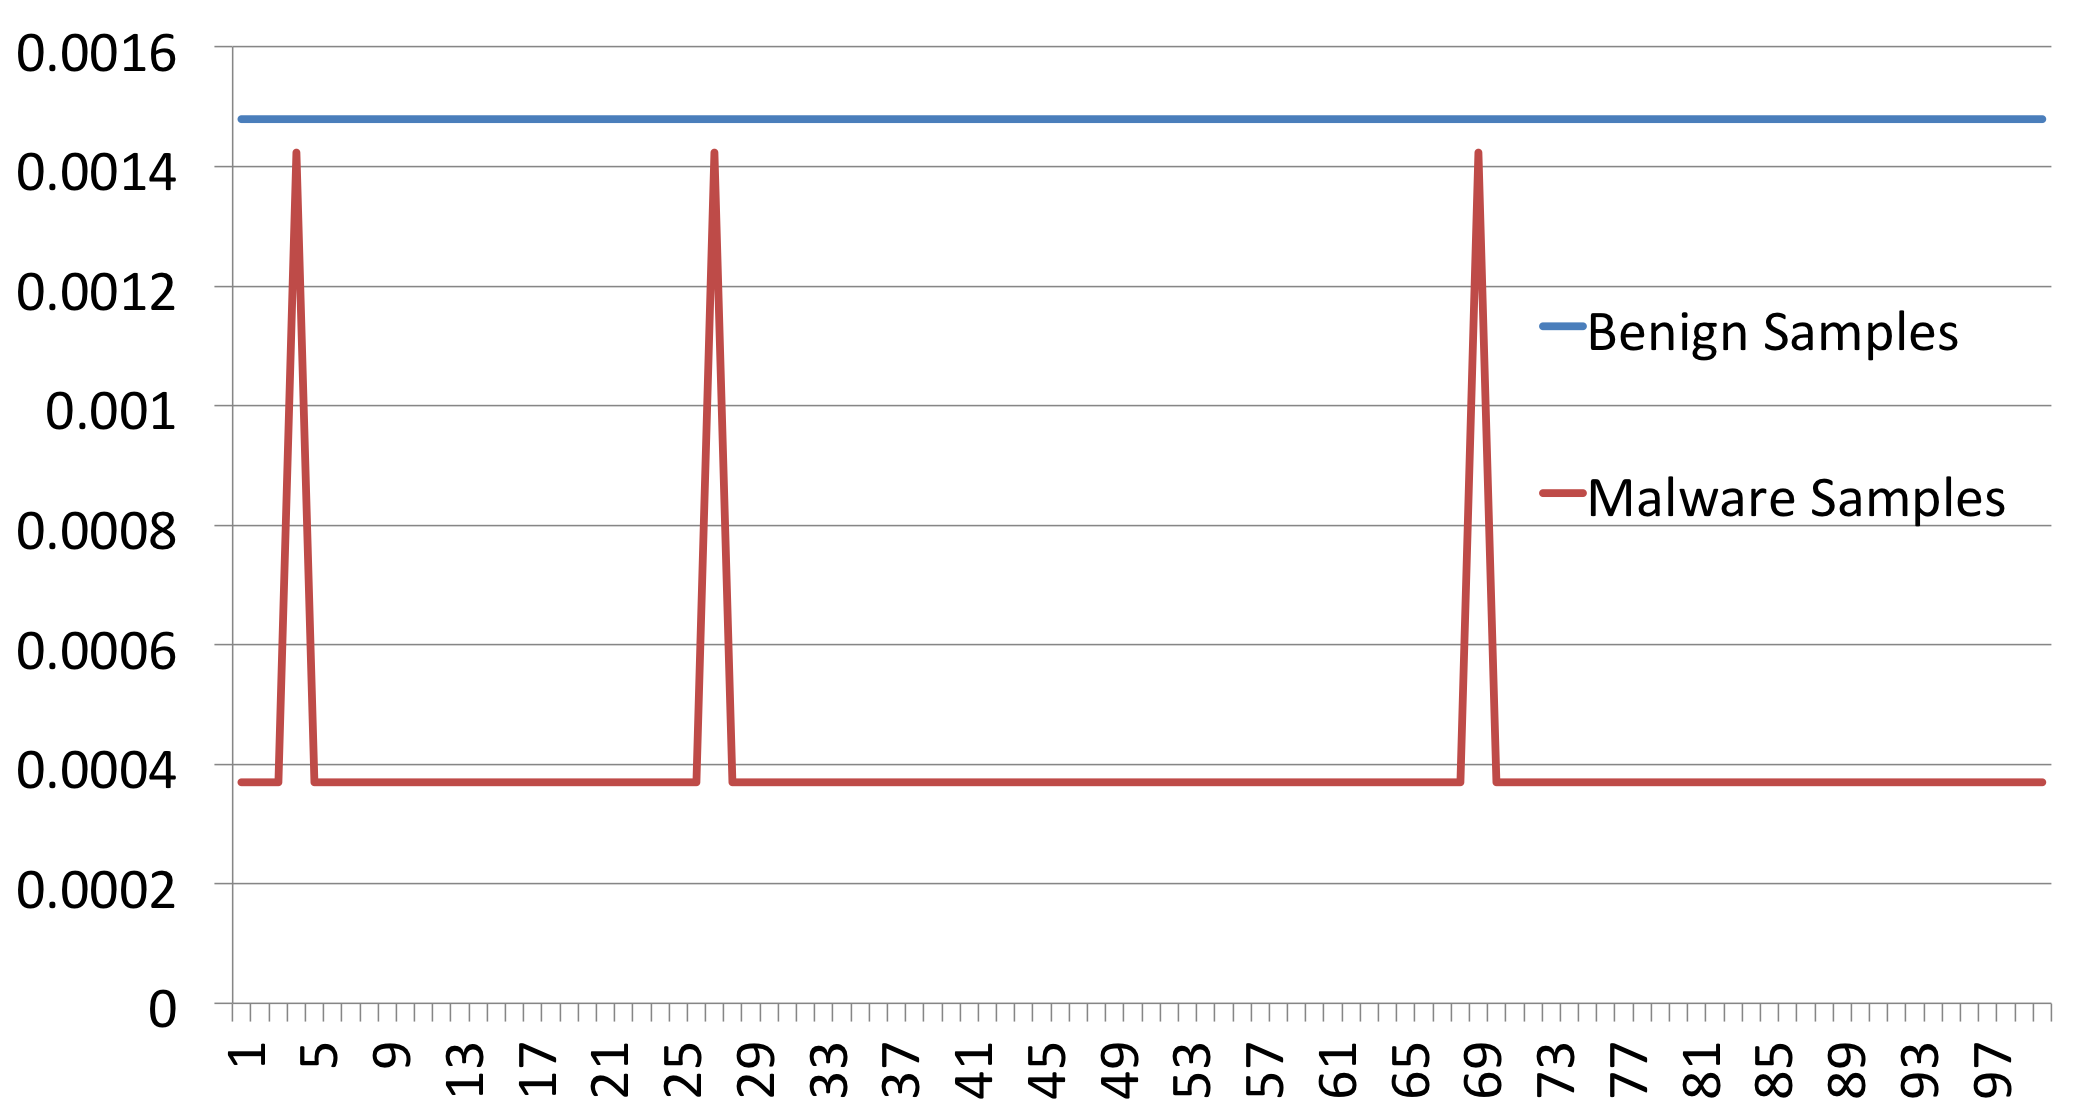
\includegraphics[width=16cm, height=9.53cm]{500.png}
    \caption[Benign Samples vs Malware Samples]{Benign samples scores vs malware samples scores with the addition of 550 lines of dead code}
    \label{fig:bvsm500}
\end{figure}


\subsection{Addition of 5500 lines of dead code}
This experiment is same as the above experiment except that here 5500 lines of dead code was included in malware and benign web pages instead of 500 lines. Tables in Figures ~\ref{fig:b5500table} and  ~\ref{fig:m5500table} contains the details of scores and execution time for this experiment. From the table values, we can see that the scores for benign web pages and malware web pages are still in the order of $10^{-3}$ and $10^{-4}$, respectively. Graph in Figure ~\ref{fig:bvsm5500} clearly shows that even after adding 5500 lines of code, the add-on is able to distinguish malware web pages and benign web pages correctly. Only 3 out of 100 malware samples have score similar to benign web pages.

\begin{figure}[h]
  \centering
  \begin{tabular}{|c|c|c|c|c|c|c|c|c|c|c|c|} 
  \midrule
 \begin{sideways}Score\end{sideways}& \begin{sideways}Time\end{sideways} \begin{sideways} (milliseconds)\end{sideways}& \begin{sideways}Score\end{sideways}& \begin{sideways}Time\end{sideways}  \begin{sideways}(milliseconds)\end{sideways}& \begin{sideways}Score\end{sideways}& \begin{sideways}Time\end{sideways}  \begin{sideways}(milliseconds)\end{sideways}& \begin{sideways}Score\end{sideways}& \begin{sideways}Time\end{sideways}  \begin{sideways} (milliseconds)\end{sideways}\\
\midrule
0.0014792907&2287&0.0014792903&1937&0.00147929&2379&0.0014792903&3148\\
\midrule
0.00147929&2447&0.0014792893&2813&0.0014792896&1966&0.0014792907&2210\\
\midrule
0.00147929&2215&0.0014792903&2153&0.0014792903&2728&0.0014792903&2094\\
\midrule
0.0014792907&2376&0.0014792903&2604&0.00147929&2167&0.0014792903&2068\\
\midrule
0.00147929&2188&0.0014792914&2221&0.0014792903&2022&0.0014792907&2462\\
\midrule
0.0014792903&2661&0.00147929&2152&0.0014792907&2383&0.0014792893&2060\\
\midrule
0.0014792907&1989&0.0014792903&2404&0.0014792903&2033&0.00147929&2074\\
\midrule
0.00147929&2137&0.00147929&2260&0.00147929&2463&0.0014792903&2254\\
\midrule
0.0014792903&2001&0.0014792907&2110&0.0014792903&2535&0.0014792893&2564\\
\midrule
0.0014792907&2003&0.0014792893&2226&0.0014792903&2026&0.0014792903&2084\\
\midrule
0.00147929&2646&0.0014792903&2134&0.0014792907&2030&0.0014792903&2406\\
\midrule
0.0014792903&1969&0.0014792903&2115&0.0014792907&1944&0.0014792903&2437\\
\midrule
0.0014792903&1972&0.0014792903&2003&0.0014792893&2239&0.0014792889&2317\\
\midrule
0.0014792903&1937&0.0014792893&1989&0.0014792893&2270&0.0014792903&2001\\
\midrule
0.0014792903&1992&0.00147929&2599&0.00147929&1954&0.0014792903&1933\\
\midrule
0.0014792896&2612&0.0014792893&2277&0.0014792907&1961&0.00147929&1994\\
\midrule
0.0014792903&2092&0.0014792896&1971&0.0014792893&2240&0.0014792903&1967\\
\midrule
0.0014792907&2453&0.0014792903&2388&0.0014792907&2280&0.00147929&2279\\
\midrule
0.0014792903&2028&0.00147929&1983&0.00147929&1966&0.0014792903&1968\\
\midrule
0.00147929&2018&0.0014792903&1996&0.0014792903&1985&0.001479291&1978\\
\midrule
0.0014792903&2010&0.0014792903&1990&0.00147929&1978&0.0014792907&1946\\
\midrule
0.0014792896&1981&0.0014792903&2034&0.00147929&1995&0.0014792903&1980\\
\midrule
0.0014792893&1967&0.00147929&1980&0.0014792907&1987&0.00147929&1942\\
\midrule
0.0014792903&1938&0.0014792903&2005&0.00147929&1962&0.00147929&1989\\
\midrule
0.0014792896&2324&0.0014792903&2103&0.0014792907&2497&0.0014792903&1985\\
\midrule
\end{tabular}
    \caption[Scores table of benign web pages]{Table illustrating the scores and add-on execution time for 100 benign web pages, in four columns (i.e., 25 samples per column). Benign webpages are generated with 5500 lines of dead code.}
    \label{fig:b5500table}
\end{figure}
\begin{figure}[h]
  \centering
  \begin{tabular}{|c|c|c|c|c|c|c|c|c|c|c|c|} 
  \midrule
 \begin{sideways}Score\end{sideways}& \begin{sideways}Time\end{sideways} \begin{sideways} (milliseconds)\end{sideways}& \begin{sideways}Score\end{sideways}& \begin{sideways}Time\end{sideways}  \begin{sideways}(milliseconds)\end{sideways}& \begin{sideways}Score\end{sideways}& \begin{sideways}Time\end{sideways}  \begin{sideways}(milliseconds)\end{sideways}& \begin{sideways}Score\end{sideways}& \begin{sideways}Time\end{sideways}  \begin{sideways} (milliseconds)\end{sideways}\\
\midrule
0.00036982243&8233&0.00036982243&8232&0.0003698225&8499&0.00036982258&7472\\
\midrule
0.0003698225&7442&0.0014239947&8681&0.0003698225&7973&0.00036982226&8276\\
\midrule
0.0003698225&7297&0.0003698225&6720&0.0003698224&8310&0.00036982235&8916\\
\midrule
0.0014239941&7827&0.0003698225&7818&0.00036982258&7843&0.00036982243&7925\\
\midrule
0.00036982258&7850&0.00036982258&8466&0.00036982258&7476&0.00036982258&7405\\
\midrule
0.00036982247&8132&0.00036982243&7717&0.00036982234&7933&0.0003698224&8014\\
\midrule
0.00036982258&8478&0.0003698225&9749&0.00036982258&7844&0.0003698225&8181\\
\midrule
0.0003698225&8910&0.00036982243&7992&0.00036982234&9089&0.0003698225&7358\\
\midrule
0.0003698224&7029&0.0003698225&7495&0.00036982243&7412&0.00036982266&7505\\
\midrule
0.00036982234&8039&0.00036982258&7474&0.0003698225&9174&0.00036982275&8958\\
\midrule
0.00036982234&7937&0.00036982243&7743&0.0003698225&7246&0.00036982258&8510\\
\midrule
0.00036982258&8008&0.00036982266&7970&0.0003698225&7440&0.0003698225&7740\\
\midrule
0.00036982243&8012&0.00036982266&8106&0.00036982258&8472&0.00036982258&8390\\
\midrule
0.00036982257&7884&0.00036982258&7892&0.0003698224&7832&0.00036982258&8352\\
\midrule
0.00036982241&8593&0.0003698225&7070&0.0003698225&6720&0.00036982243&8671\\
\midrule
0.00036982249&8147&0.0003698225&7188&0.00036982243&8236&0.0003698224&8519\\
\midrule
0.0003698225&7143&0.00036982232&8449&0.00036982258&8064&0.0003698225&6830\\
\midrule
0.0003698225&8747&0.00036982266&7731&0.00036982243&8323&0.0003698224&8421\\
\midrule
0.00036982258&7226&0.00036982258&8379&0.0014239943&7039&0.00036982243&8282\\
\midrule
0.00036982258&7001&0.00036982243&9518&0.00036982251&7213&0.00036982249&7813\\
\midrule
0.00036982249&6871&0.00036982249&9287&0.00036982243&9476&0.00036982252&8132\\
\midrule
0.00036982243&7892&0.00036982252&8936&0.00036982266&8468&0.0003698224&7930\\
\midrule
0.0003698225&7989&0.0003698224&8250&0.00036982243&8304&0.0003698225&7418\\
\midrule
0.00036982234&7814&0.0003698224&8658&0.00036982258&7766&0.0003698225&9372\\
\midrule
0.0003698225&8370&0.00036982258&8248&0.00036982258&7644&0.00036982266&8933\\
\midrule
\end{tabular}
    \caption[Scores table of malware web pages]{Table illustrating the scores and add-on execution time for 100 malware web pages, in four columns (i.e., 25 samples per column). Malware webpages are morphed with 5500 lines of dead code. }
    \label{fig:m5500table}
\end{figure}

\begin{figure}[h]
    \centering    
    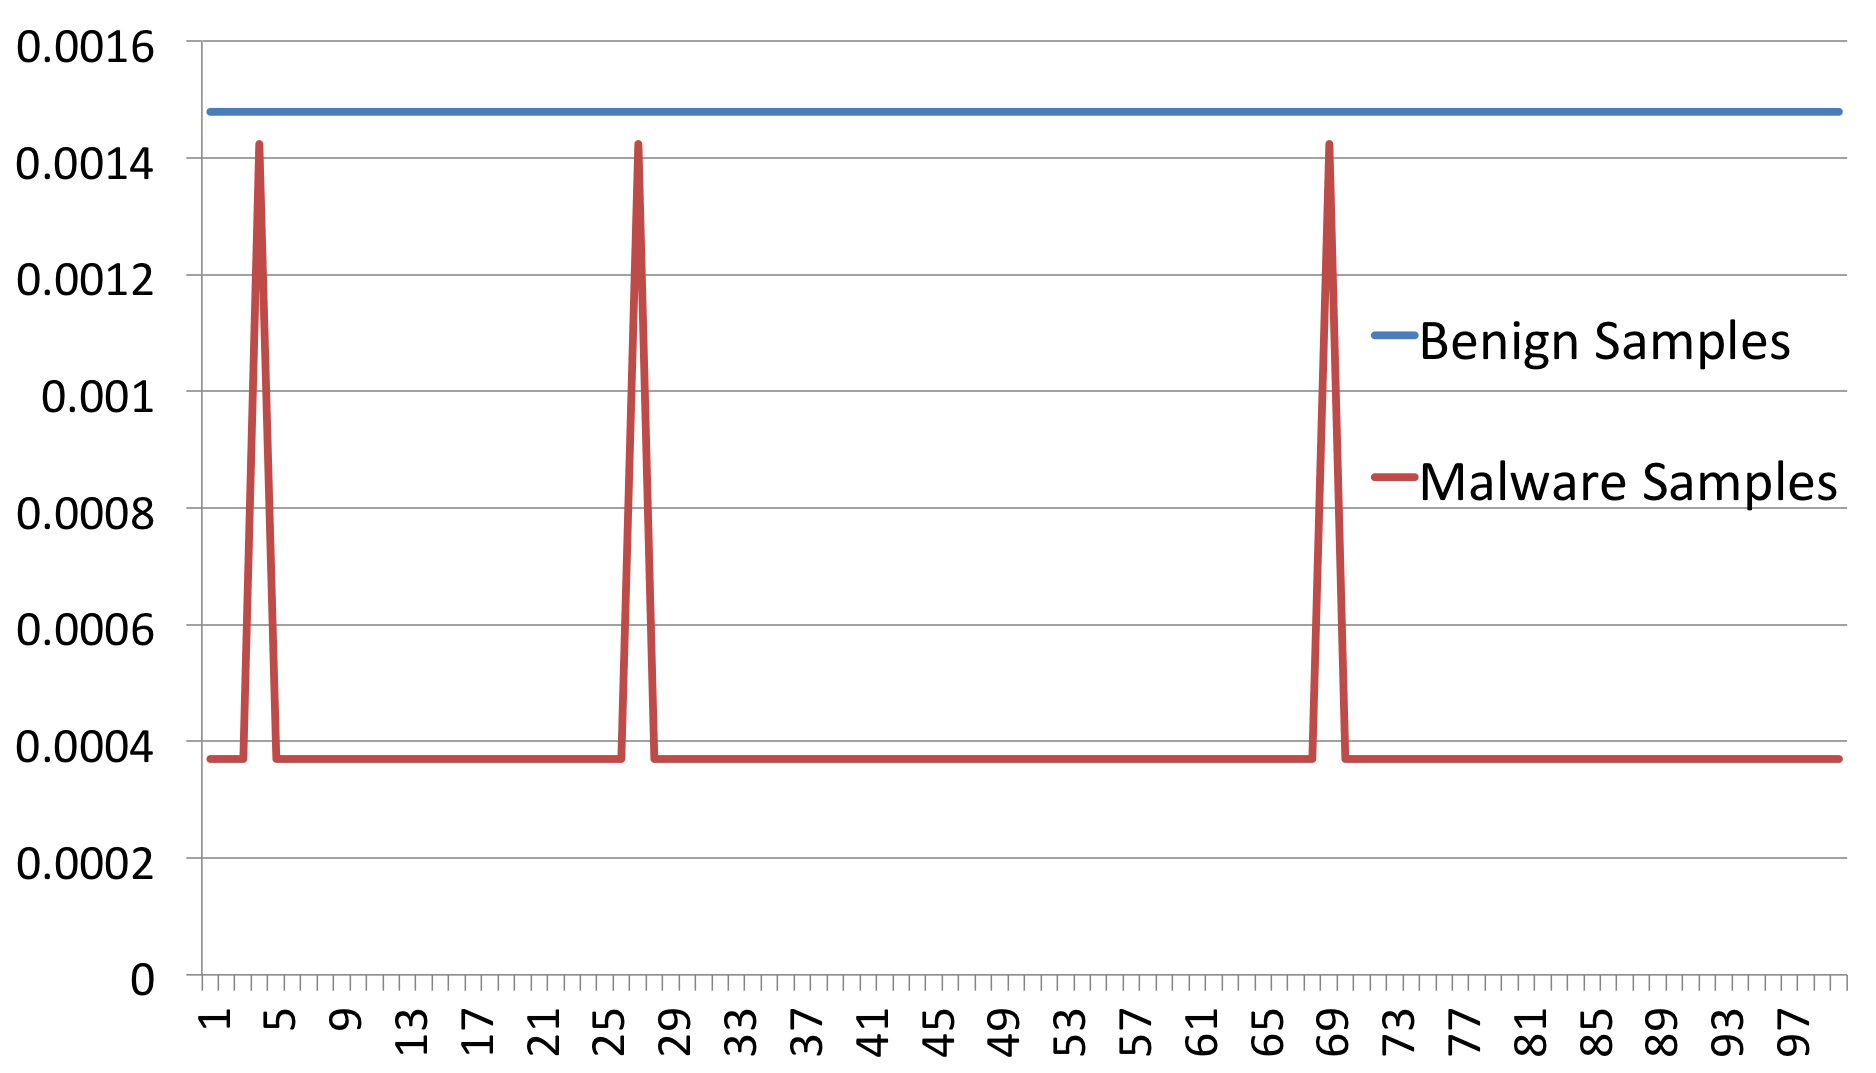
\includegraphics[width=16cm, height=10cm]{5000.png}
    \caption[Benign Samples vs Malware Samples]{Benign samples scores vs malware samples scores with the addition of 5500 lines of dead code}
    \label{fig:bvsm5500}
\end{figure}

\subsection{Addition of 15000 lines of dead code}
Here, 15000 lines of dead code was included in malware and benign samples. From the tables in Figures ~\ref{fig:b15000table} and  ~\ref{fig:m15000table}, it is clear that scores of malware web pages are varied by very negligible value when compared to previous experiments. So as shown in Figure ~\ref{fig:bvsm15000}, add-on is still able to distinguish malware web pages and benign web pages correctly.

\begin{figure}[h]
  \centering
  \begin{tabular}{|c|c|c|c|c|c|c|c|c|c|c|c|} 
  \midrule
 \begin{sideways}Score\end{sideways}& \begin{sideways}Time\end{sideways} \begin{sideways} (milliseconds)\end{sideways}& \begin{sideways}Score\end{sideways}& \begin{sideways}Time\end{sideways}  \begin{sideways}(milliseconds)\end{sideways}& \begin{sideways}Score\end{sideways}& \begin{sideways}Time\end{sideways}  \begin{sideways}(milliseconds)\end{sideways}& \begin{sideways}Score\end{sideways}& \begin{sideways}Time\end{sideways}  \begin{sideways} (milliseconds)\end{sideways}\\
\midrule
0.0014792903&3241&0.001479291&3301&0.0014792903&3274&0.0014792903&3484\\
\midrule
0.0014792903&3180&0.00147929&3162&0.00147929&3355&0.0014792896&3342\\
\midrule
0.00147929&3172&0.0014792896&3134&0.00147929&3345&0.0014792903&3415\\
\midrule
0.0014792893&3291&0.0014792903&3150&0.00147929&3185&0.0014792896&3409\\
\midrule
0.001479291&3161&0.0014792896&3545&0.0014792907&3184&0.0014792896&3536\\
\midrule
0.0014792903&3178&0.00147929&3104&0.00147929&3445&0.00147929&3540\\
\midrule
0.0014792907&3182&0.00147929&3167&0.0014792896&4519&0.0014792903&3794\\
\midrule
0.00147929&3378&0.0014792896&3307&0.00147929&3448&0.0014792896&3786\\
\midrule
0.00147929&3575&0.0014792907&3192&0.0014792907&3361&0.0014792896&3696\\
\midrule
0.00147929&3563&0.0014792896&3131&0.00147929&3181&0.0014792896&3513\\
\midrule
0.0014792903&3271&0.0014792903&3216&0.0014792903&3383&0.0014792903&3405\\
\midrule
0.0014792907&3188&0.0014792889&3320&0.0014792903&4725&0.0014792907&3608\\
\midrule
0.0014792903&3122&0.0014792896&3137&0.0014792903&3602&0.00147929&3275\\
\midrule
0.00147929&3467&0.0014792903&3225&0.0014792907&3217&0.0014792893&3439\\
\midrule
0.0014792903&3197&0.0014792903&3328&0.00147929&3464&0.00147929&3700\\
\midrule
0.0014792907&3149&0.0014792903&3329&0.00147929&3159&0.0014792907&3230\\
\midrule
0.0014792893&3139&0.00147929&3201&0.0014792903&4870&0.00147929&3221\\
\midrule
0.0014792893&3100&0.0014792896&3171&0.0014792896&3244&0.0014792907&3199\\
\midrule
0.00147929&3206&0.0014792903&4664&0.00147929&3292&0.0014792896&3239\\
\midrule
0.0014792903&3139&0.00147929&3105&0.00147929&3417&0.00147929&3133\\
\midrule
0.0014792896&3159&0.0014792893&3177&0.0014792903&3341&0.0014792903&3300\\
\midrule
0.001479291&3102&0.00147929&3467&0.00147929&4321&0.0014792903&3420\\
\midrule
0.0014792903&3267&0.0014792903&3426&0.00147929&3587&0.0014792896&5329\\
\midrule
0.00147929&3359&0.00147929&3421&0.0014792893&3333&0.0014792907&3614\\
\midrule
0.0014792903&3412&0.00147929&3400&0.001479291&3289&0.0014792903&3450\\
\midrule
\end{tabular}
    \caption[Scores table of benign web pages]{Table illustrating the scores and add-on execution time for 100 benign web pages, in four columns (i.e., 25 samples per column). Benign webpages are generated with 15000 lines of dead code.}
    \label{fig:b15000table}
\end{figure}
\begin{figure}[h]
  \centering
  \begin{tabular}{|c|c|c|c|c|c|c|c|c|c|c|c|} 
  \midrule
 \begin{sideways}Score\end{sideways}& \begin{sideways}Time\end{sideways} \begin{sideways} (milliseconds)\end{sideways}& \begin{sideways}Score\end{sideways}& \begin{sideways}Time\end{sideways}  \begin{sideways}(milliseconds)\end{sideways}& \begin{sideways}Score\end{sideways}& \begin{sideways}Time\end{sideways}  \begin{sideways}(milliseconds)\end{sideways}& \begin{sideways}Score\end{sideways}& \begin{sideways}Time\end{sideways}  \begin{sideways} (milliseconds)\end{sideways}\\
\midrule
0.00036982258&9192&0.0003698224&9179&0.0003698225&9225&0.00036982266&8274\\
\midrule
0.00036982258&9105&0.0003698225&7719&0.0003698225&9240&0.00036982258&8962\\
\midrule
0.0003698225&9104&0.00036982258&8207&0.0003698225&9458&0.00036982263&9132\\
\midrule
0.0003698225&9303&0.00036982243&9510&0.00036982266&8810&0.0003698225&8588\\
\midrule
0.00036982258&8568&0.00036982258&9779&0.00036982243&8545&0.0003698224&8185\\
\midrule
0.00036982241&9942&0.0003698225&9537&0.0014239943&8158&0.0003698224&8915\\
\midrule
0.00036982266&9502&0.00036982266&9766&0.00036982258&8540&0.00036982266&9395\\
\midrule
0.0003698224&9791&0.0003698225&8802&0.0003698225&9080&0.00036982258&8165\\
\midrule
0.0003698225&7951&0.00036982243&10122&0.00036982258&9233&0.00036982234&8113\\
\midrule
0.0003698225&8565&0.0003698225&9180&0.0003698224&8556&0.0003698225&9760\\
\midrule
0.0003698225&8059&0.00036982234&8254&0.0003698224&9702&0.0003698224&9330\\
\midrule
0.0003698225&8889&0.00036982258&8146&0.00036982258&9082&0.00036982258&8756\\
\midrule
0.0003698225&8884&0.00036982258&7851&0.0003698225&9281&0.0003698225&9336\\
\midrule
0.00036982235&9126&0.00036982258&8672&0.00036982258&8465&0.0003698225&8828\\
\midrule
0.00036982251&9631&0.00036982258&7948&0.00036982258&9770&0.00036982258&9277\\
\midrule
0.0003698226&8128&0.00036982266&8689&0.00036982258&9211&0.0003698225&9478\\
\midrule
0.00036982243&7919&0.0003698225&8264&0.00036982243&9809&0.00036982258&7847\\
\midrule
0.0003698225&9433&0.0003698225&8562&0.0003698224&9109&0.00036982266&9312\\
\midrule
0.0003698225&8202&0.00036982258&8119&0.001423994&9592&0.00036982266&8933\\
\midrule
0.00036982243&8400&0.00036982266&8845&0.0014239942&1070&0.00036982249&9612\\
\midrule
0.00036982252&9783&0.00036982266&8845&0.00036982266&9750&0.00036982258&8495\\
\midrule
0.00036982258&8811&0.00036982266&8845&0.00036982243&9469&0.0003698224&8855\\
\midrule
0.00036982275&10339&0.0003698225&9078&0.0003698224&8303&0.00036982258&7895\\
\midrule
0.0003698225&8925&0.00036982258&9246&0.00036982258&8821&0.0003698224&10477\\
\midrule
0.00036982243&9367&0.0003698224&8687&0.00036982258&8830&0.00036982243&8510\\
\midrule
\end{tabular}
    \caption[Scores table of malware web pages]{Table illustrating the scores and add-on execution time for 100 malware web pages, in four columns (i.e., 25 samples per column). Malware web pages are morphed with 15000 lines of dead code. }
    \label{fig:m15000table}
\end{figure}

\begin{figure}[h]
    \centering    
    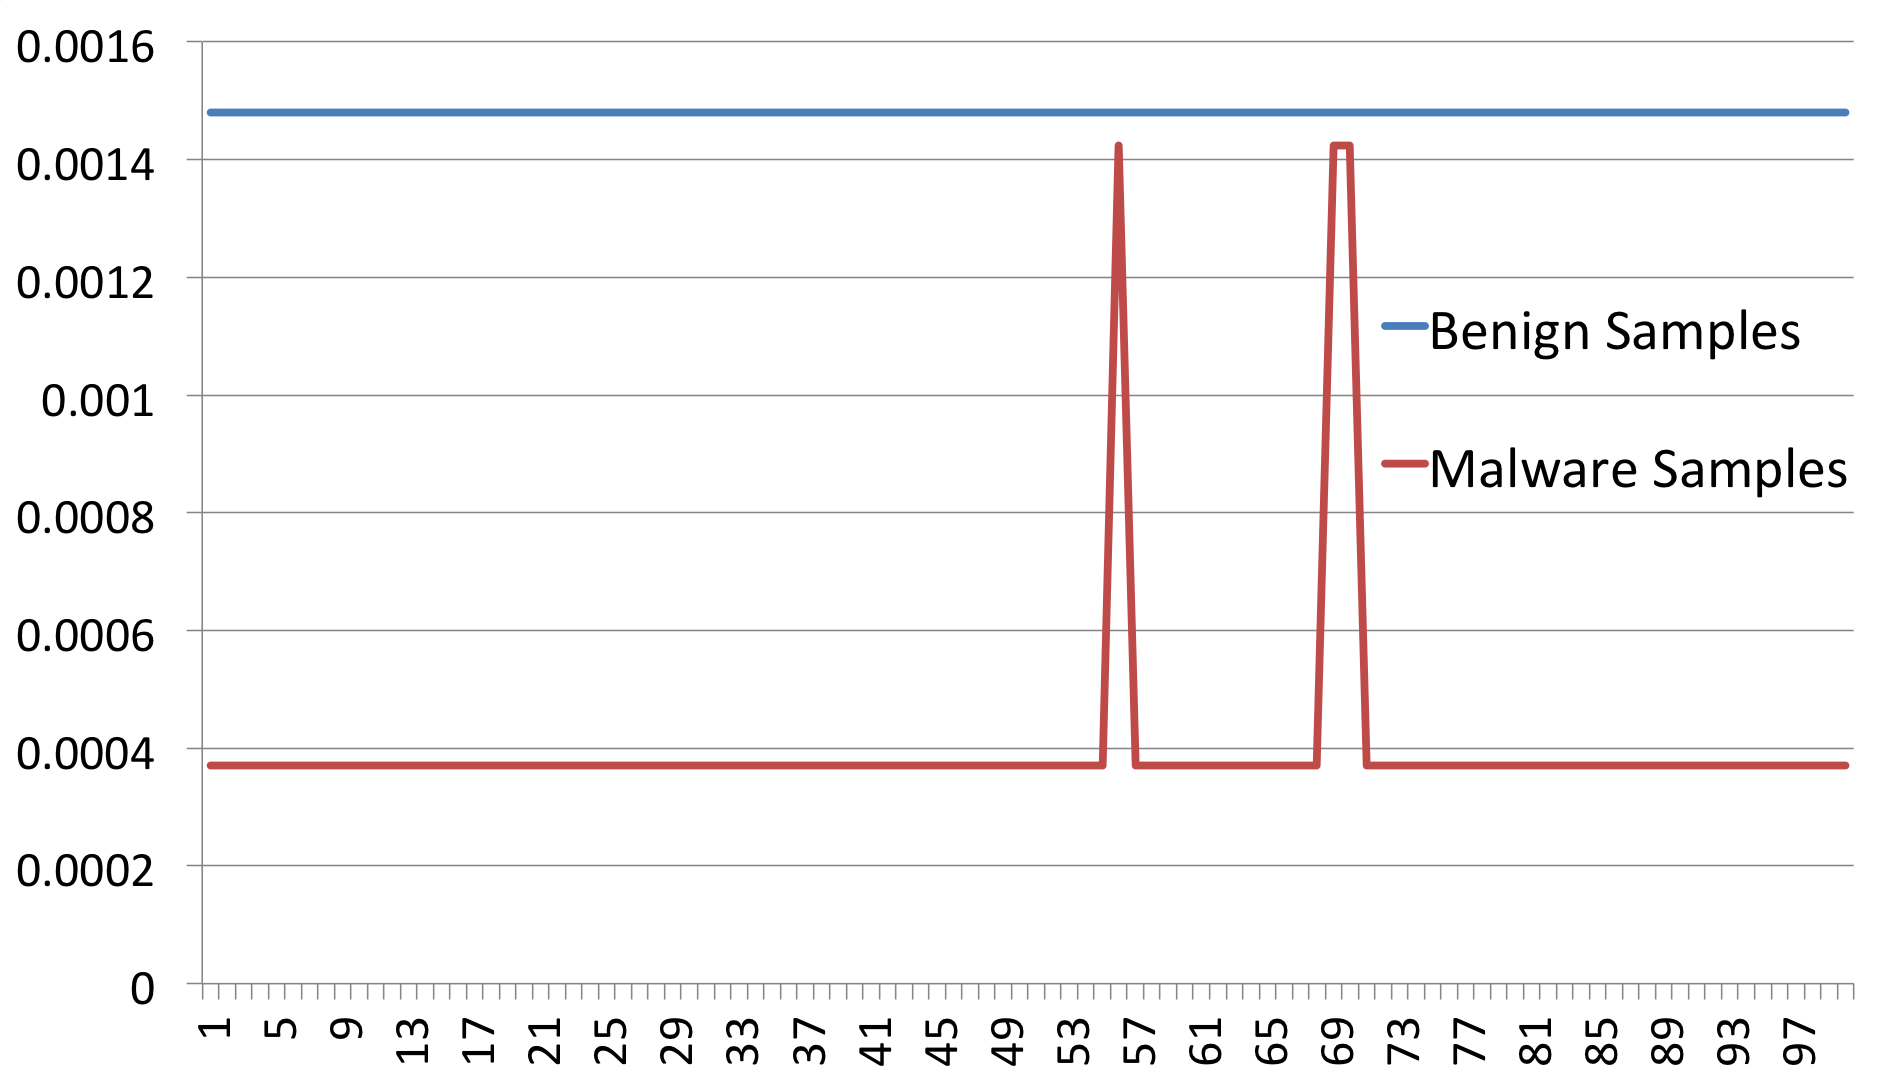
\includegraphics[width=16cm, height=10.30cm]{15000.png}
    \caption[Benign Samples vs Malware Samples]{Benign samples scores vs malware samples scores with the addition of 15000 lines of dead code}
    \label{fig:bvsm15000}
\end{figure}

As mentioned in Section \ref{opcodescorecalculation}, the scores of malware files and benign files can be compared to calculate the threshold score value of the opcode similarity technique. From the tables in Figures ~\ref{fig:b500table}, ~\ref{fig:b5500table}, ~\ref{fig:b15000table}, ~\ref{fig:m500table}, ~\ref{fig:m5500table}, and ~\ref{fig:m15000table}, except 9 malwares all other malware scores are in between $0.000369822260$ and $0.000369822750$. The 9 exception malware scores are between $0.001423994000$ and $0.001423994700$. And the benign web page scores are between $0.001479288900$ and $0.001479291400$. The same information is represented with table in Figure ~\ref{fig:scoresummarytable}


\begin{figure}[h]
  \centering
  \begin{tabular}{|c|c|c|} 
  \midrule
 & Min Score& Max Score\\
\midrule
291 malware samples & 0.000369822260 & 0.000369822750\\ 
 \midrule 
9 exceptional malware samples & 0.001423994000 & 0.001423994700\\ 
 \midrule 
300 Benign samples &0.001479288900 & 0.001479291400 \\
 \midrule 
\end{tabular}
    \caption[Summary of max and min Scores]{Table illustrating the max and min scores for all the sample files, after comparing the scores from the tables in Figures ~\ref{fig:b500table}, ~\ref{fig:b5500table}, ~\ref{fig:b15000table}, ~\ref{fig:m500table}, ~\ref{fig:m5500table}, and ~\ref{fig:m15000table}. }
    \label{fig:scoresummarytable}
\end{figure}

Threshold value can be any value between 0.00142 and 0.00147. If the less percentage of false negative rate is acceptable, then the threshold score can be choosen between 0.00036 and 0.00147. In case of malware detection, it is always better to have less negative rate, so considered \textbf{0.00145} as threshold score value for the add-on.

\section{Test for False Positive rate of the add-on}

Tested the add-on on popular web sites to detect "False Positive" rate of the add-on. Popular web site links are retrieved from http://en.wikipedia.org/wiki/List\_of\_most\_popular\_websites. 

Table in Figure\ref{fig:scoresummarytablep}, contains the scores and execution time details. All the scores in the table are more than choosen threshold value (i.e., 0.00145), which means that the add-on validated all the web pages as benign web pages i.e., add-on has zero false positive rate.

\begin{figure}[h]
  \centering
  \begin{tabular}{|c|c|c|c|} 
  \midrule
 Web page& Score& Time (Milli seconds) & Result\\
  \midrule
https://www.google.com/&0.025195263&2189&Benign page\\
\midrule
https://www.facebook.com/&0.08652405&3190&Benign page\\
\midrule
http://www.baidu.com/&0.051652893&4442&Benign page\\
\midrule
http://www.twitter.com/&0.8132002&4076&Benign page\\
\midrule
http://www.taobao.com&0.29001402&3401&Benign page\\
\midrule
http://www.qq.com/&0.014076417&3177&Benign page\\
\midrule
https://www.linkedin.com&0.0916255&4309&Benign page\\
\midrule
https://live.com&0.30142236&1379&Benign page\\
\midrule
http://www.sina.com.cn/&0.04421566&2513&Benign page\\
\midrule
http://us.weibo.com/gb&0.210642001&2921&Benign page\\
\midrule
http://www.hao123.com/&0.046390533&5314&Benign page\\
\midrule
http://www.bing.com/&0.30142236&1323&Benign page\\
\midrule
http://www.apple.com/&0.0625&5505&Benign page\\
\midrule
http://www.aliexpress.com/&0.06497499&1794&Benign page\\
\midrule
http://www.imdb.com/&0.041259766&8022&Benign page\\
\midrule
http://www.alibaba.com/&0.0047562416&3206&Benign page\\
\midrule
http://www.ask.com/&0.051652893&4611&Benign page\\
\midrule
https://www.netflix.com&0.0625&10046&Benign page\\
\midrule
http://www.naver.com/&0.30142236&2504&Benign page\\
\midrule
http://diply.com/&0.05702829&8612&Benign page\\
\midrule
https://mail.google.com&0.30142236&1713&Benign page\\
\midrule
http://www.youku.com/&0.051652893&4044&Benign page\\
\midrule
http://www.flipkart.com/&0.018838914&1604&Benign page\\
\midrule
https://www.amazon.com/&0.100754&2839&Benign page\\
\midrule
http://www.wikipedia.org/&0.094681033&1914&Benign page\\
\midrule
\end{tabular}
    \caption[Scores table for popular web pages]{Table contains scores and add-on exection time details for popular web pages. }
    \label{fig:scoresummarytablep}
\end{figure}

\section{Splitting Transcriptase code}

Transcriptase can be split into several external JS files and then the external files can be included in a web page. So, the following experiment was performed to calculate the scores of split files by dividing the Transcriptase in to various number of files.

Code was split based on Functions count. The experiment was started by dividing the Transcriptase code into two files with almost equal number of functions and then continued till the split files count reaches 76. A parser code was developed in Python to detect the valid start and end point of the JavaScript functions and to properly split the Transcriptase code. Thus the resultant split files are syntactically correct. Code \ref{lst:pythonparser} shows the parser logic in Python language.


\begin{lstlisting}[language=Python, caption={Parser code detects the valid start and end point of the JavaScript functions and properly splits the Transcriptase code.},label={lst:pythonparser}, mathescape=false]
with open("transcriptase.js", "r") as ins:
    total_functions = 1000 
    line = ins.read()
    k = sys.argv[1]        
    required = (int)(total_functions/k)
    cnt,braces,rbraces,sbraces,brackets_match,func_ind = 0,0,0,0,0,0
    skip, eachfun_done = False, False
    data, skip_char = '', ''
    function_start = True
    func = ['f','u','n','c','t','i','o','n']
    for c in line:
        if cnt == required and eachfun_done == True:
            cnt = 0
            eachfun_done = False
            #write data into a file 
            data=''
        if (c=='\textquotedblleft' or c=="\textquoteleft") and skip==False:
            skip = True
            data = data+c
            skip_char = c
            continue
        if skip == True:
            data = data+c
            if skip_char == c:
                skip = False
                skip_char = ''
            continue
        if c == '(':
            rbraces+=1
        elif c == ')':
            rbraces-=1
        if c == '[':
            sbraces+=1
        elif c == ']':
            sbraces-=1
        if c == '{':
            if function_start==True:
                function_start=False
            braces+=1
        elif c == '}':
            braces-=1
        if braces == 0 and sbraces ==0 and rbraces == 0:
            if function_start==False:
                eachfun_done = True
        else:
            data = data +c
            continue 
        if func[func_ind] == c:
            func_ind+=1
        else:
            func_ind=0
        if func_ind == 8:
            total_functions+=1
            cnt+=1
            function_start=True
            eachfun_done = False
            func_ind=0
        data+=c
    if data != "":
        cnt = 0
        eachfun_done = False
        #write data into a file 
        data=''
\end{lstlisting}

Table \ref{tab:splitvalues} shows the results for various splits. "Max" and "Min" column specifies maximum and minimum similarity score among the split files, respectively. "Count" column specifies "to number of files the Transcriptase code was split into".

Figure \ref{fig:splitgraph}, is a graphical representation of the Table \ref{tab:splitvalues} values. Graph clearly shows that even the code was split, \textbf{minumum score among the split files is always less than threshold which means that there always exists atleast one split file with score less than threshold score}. Thus, it is possible to detect the malware even by testing all the external files separately. So, we can validate all the external scripts parallely to increase the performance of the add-on.


\begin {table}[h]
\caption {Splitting Transcriptase into several files} \label{tab:splitvalues} 
  \begin{tabular}{|c|c|c|c|c|c|}  
  \midrule
 Count&Min&Max&Count&Min&Max\\
\midrule
1&3.70E-04&3.70E-04&20&1.68E-18&0.018838914\\
\midrule
2&1.28E-18&1.16E-17&21&1.81E-17&0.018838914\\
\midrule
3&1.77E-19&1.39E-17&22&1.69E-19&0.018838914\\
\midrule
4&6.17E-19&1.75E-17&23&9.64E-20&0.018838914\\
\midrule
5&4.41E-20&3.84E-04&24&7.37E-19&0.018838914\\
\midrule
6&5.36E-18&0.00153787&26&1.61E-19&0.01883891\\
\midrule
7&4.57E-19&3.84E-04&27&2.27E-17&0.018838914\\
\midrule
8&2.19E-18&0.00153787&29&9.72E-19&0.018838914\\
\midrule
9&1.86E-17&0.00153787&31&3.85E-18&0.018838914\\
\midrule
10&1.69E-19&0.003460208&33&6.35E-18&0.018838914\\
\midrule
11&1.73E-18&0.00615148&35&4.33E-18&0.018838914\\
\midrule
12&3.91E-18&0.003460208&38&4.37E-18&0.018838914\\
\midrule
13&5.64E-20&0.00615148&42&8.12E-18&0.018838914\\
\midrule
14&5.47E-19&0.003460208&46&4.41E-20&0.018838914\\
\midrule
15&1.88E-18&0.00615148&51&5.21E-18&0.018838914\\
\midrule
16&8.01E-20&0.009611688&57&1.96E-17&0.018838914\\
\midrule
17&1.26E-18&0.013840835&65&3.84E-04&0.024605926\\
\midrule
18&5.07E-19&0.009611691&76&3.84E-04&0.024605926\\
\midrule
19&8.01E-19&0.018838914\\
\cmidrule{1-3}
\end{tabular}
 \end {table}

\begin{figure}[h]
    \centering    
    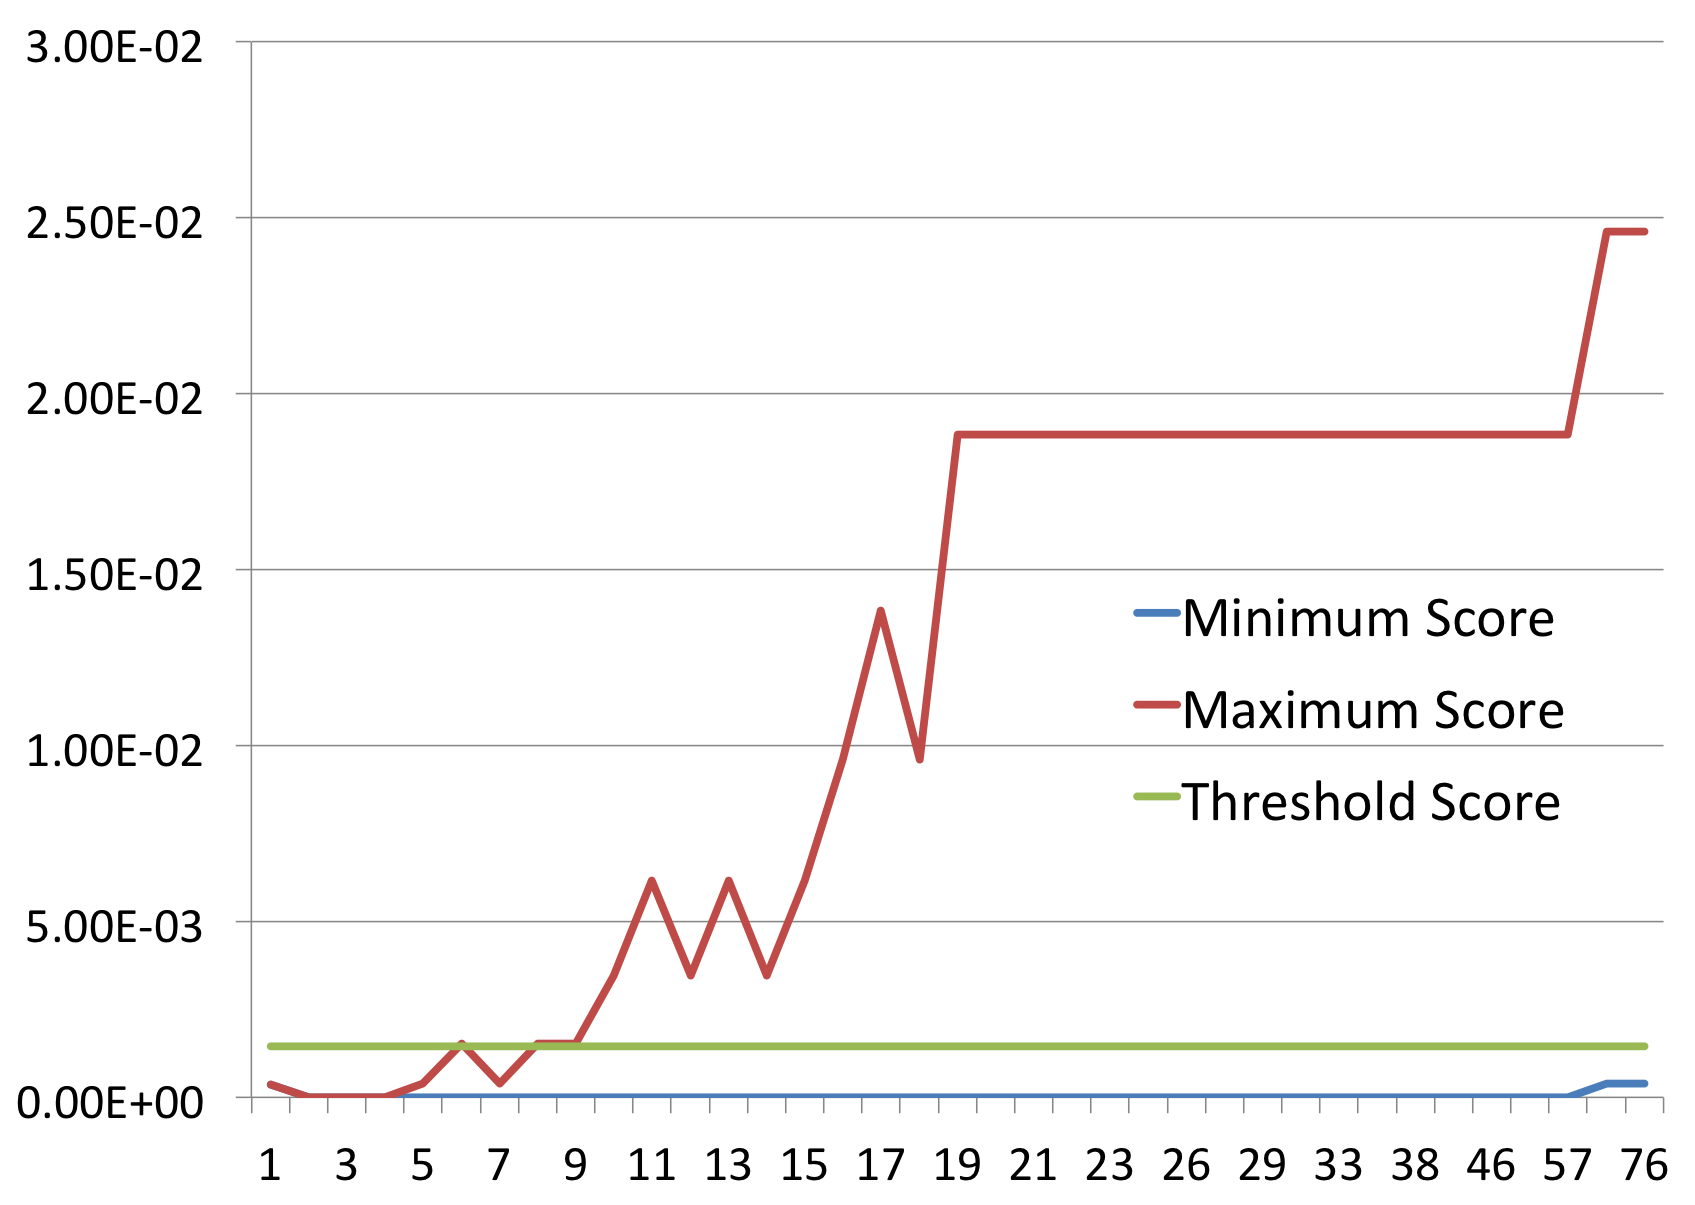
\includegraphics[width=16cm, height=13.85cm]{external.png}
    \caption[Graph showing min and max scores of split files ]{Graph showing min and max scores of Transcriptase split files.}
    \label{fig:splitgraph}
\end{figure}